%!TEX root = ../../dissertation.tex

\section{Tables and Figures}


%
% Tables
%
\subsection{Tables}

  \begin{table}[H]
    \begin{tabular}{lll}
      \toprule
      \textbf{Parameter Name} & \textbf{Value} & \textbf{Source} \\
      \midrule
      $\beta$ & 0.98 & Standard \\
      $r$ & 0.04 & \\
      \midrule
      $T$ & 42 & Retirement at 60 \\
      \midrule
      $\tau, \lambda$ & 0.118, 1.07 & \cite{HeathcoteStoreslettenViolante2017} \\
      \midrule
      $\sigma^{HS, w}, \sigma^{CD, w}, \sigma^{CG, w}$ & $\sqrt{0.011}, \sqrt{0.011}, \sqrt{0.0099}$ & \cite{Guvenen2009}, \cite{CarrollSamwick1997} \\
      $\sigma^{HS, y}, \sigma^{CD, y}, \sigma^{CG, y}$ & $\sqrt{0.052}, \sqrt{0.052}, \sqrt{0.047}$ & \\
      \midrule
      $\phi_{HS}, \phi_{CD}, \phi_{CG}$ & 0.15, 0.15, 0.197 & \cite{HendricksLeukhina2017} \\
      $\mu, w_{\text{coll}}$ & 0.010, 3.55 & \\
      $\gamma_\text{min}, \gamma_1, \gamma_2$ & 0.47, 4.58, 2.10 & \\
      $\alpha_{am}$, $\alpha_{m,GPA}$ & 2.87, 1.2 & \\
      $\alpha_{kq}$, $\alpha_{mq}$, $\alpha_{mz}$, $\alpha_{qz}$ & 0.0, -0.04, 0.46, -0.12 & \\
      $\mu_q$, $\sigma_q$ & 0.53, 0.35 & \\
      $\mu_z$, $\sigma_z$ & 0.32, 0.55 & \\
      \bottomrule
    \end{tabular}
    \caption{Previous Knowledge Parameters}
    \label{table:pk}
  \end{table}

  \begin{table}[H]
    \begin{tabular}{lll}
      \toprule
      \textbf{Parameter Name} & \textbf{Value} & \textbf{Source} \\
      \midrule
      $\bar{\theta}^{HS}$, $\bar{\theta}^{CG}$ & 8.73, 5.06 & \cite{PSID} \\
      $\theta_1^{HS}$, $\theta_2^{HS}$, $\theta_3^{HS}$ & 0.066, -0.088, 0.002 & \\
      $\theta_1^{CG}$, $\theta_2^{CG}$, $\theta_3^{CG}$ & 0.324, -0.624, 0.039 & \\
      \midrule
      $\bar{T}_C$ & 6 & College features \\
      $n_c$ & 6 & \\
      $n_{\text{grad}}$ & 21 & \\
      $\underbar{d}$, $\underbar{D}$ & -0.5, -1.975 & \\
      \bottomrule
    \end{tabular}
    \caption{Externally Calibrated Parameters}
    \label{table:ec}
  \end{table}

  \begin{table}[H]
    \begin{tabular}{lll}
      \toprule
      \textbf{Parameter Name} & \textbf{Value} & \textbf{Target} \\
      \midrule
      $\delta_c$, $\delta_v$ & 0.62, 1.15 & Debt accumulation \\
      $U_{HS}$, $U_{CD}$, $U_{CG}$ & 0.0, -2.97, -6.81 & Enrollment \\
      $\alpha_{km}$, $\mu_k$, $\sigma_k$ & 0.55, 2.57, 3.94 & Fraction with debt \\
      $\pi_e$, $\pi_c$ & 0.30, 1.58 & Enrollment and dropout \\
      \bottomrule
    \end{tabular}
    \caption{Internally Calibrated Parameters}
    \label{table:ic}
  \end{table}

  \begin{table}[H]
    \begin{tabular}{lccll}
      \toprule
      \multicolumn{3}{c}{\textbf{Moment Descriptions}} & \textbf{Data} & \textbf{Model} \\
      \midrule
      \textbf{Name} & \textbf{Year} & \textbf{GPA Quartile} & & \\
      \midrule
      Time to degree & --- & --- & 4.45 & 4.73 \\
      Education Fraction (HS) & --- & --- & 0.52 & 0.53 \\
      Education Fraction (CD) & --- & --- & 0.23 & 0.21 \\
      Education Fraction (CG) & --- & --- & 0.25 & 0.26 \\
      \midrule
      Enrollment & --- & Quartile 1 & 0.22 & 0.18 \\
                 & --- & Quartile 2 & 0.35 & 0.35 \\
                 & --- & Quartile 3 & 0.55 & 0.55 \\
                 & --- & Quartile 4 & 0.81 & 0.81 \\
      \midrule
      Completion & --- & Quartile 1 & 0.02 & 0.03 \\
                 & --- & Quartile 2 & 0.08 & 0.13 \\
                 & --- & Quartile 3 & 0.28 & 0.30 \\
                 & --- & Quartile 4 & 0.60 & 0.60 \\
      \midrule
      College Earnings & --- & Quartile 1 & 0.65 & 0.85 \\
                       & --- & Quartile 2 & 0.58 & 0.70 \\
                       & --- & Quartile 3 & 0.54 & 0.59 \\
                       & --- & Quartile 4 & 0.51 & 0.43 \\
      \midrule
      Average debt & Year 1 & --- & 0.35 & 0.33 \\
                   & Year 2 & --- & 0.59 & 0.50 \\
                   & Year 3 & --- & 0.78 & 0.75 \\
                   & Year 4 & --- & 0.95 & 1.06 \\
      \midrule
      Fraction with debt & Year 1 & --- & 0.26 & 0.11 \\
                         & Year 2 & --- & 0.34 & 0.27 \\
                         & Year 3 & --- & 0.41 & 0.42 \\
                         & Year 4 & --- & 0.48 & 0.52 \\
      \midrule
      Drop out & Year 1 & --- & 0.16 & 0.15 \\
               & Year 2 & --- & 0.14 & 0.10 \\
               & Year 3 & --- & 0.08 & 0.07 \\
               & Year 4 & --- & 0.05 & 0.05 \\
               & Year 5 & --- & 0.02 & 0.03 \\
      \bottomrule
    \end{tabular}
    \caption{Data and model moments}
    \label{table:moments}
  \end{table}

  \begin{table}[H]
    \begin{tabular}{llll}
      \toprule
      & \textbf{AMR} & \textbf{LC} & \textbf{IDR} \\
      \midrule
      Enrollment rate & 0.48 & 0.48 & 0.49 \\
      Completion rate & 0.27 & 0.27 & 0.27 \\
      Graduation rate & 0.56 & 0.56 & 0.56 \\
      \bottomrule
    \end{tabular}
    \caption{Student outcomes under different versions of our economy}
    \label{table:students}
  \end{table}

  \begin{table}[H]
    \begin{tabular}{llll}
      \toprule
      & \textbf{AMR} & \textbf{LC} & \textbf{IDR} \\
      \midrule
      Fraction with debt & 0.46 & 0.46 & 0.70 \\
      Average debt & \$11,750 & \$11,750 & \$13,740 \\
      \bottomrule
    \end{tabular}
    \caption{Student debt decisions under plans}
    \label{table:debt}
  \end{table}

  \begin{table}[H]
    \begin{tabular}{llll}
      \toprule
      & \textbf{AMR} & \textbf{LC} & \textbf{IDR} \\
      \midrule
      Subsidy rate & -0.13 & -0.12 & -0.06 \\
      Government subsidy (per person) & -\$0.085 & -\$0.077 & -\$0.072 \\
      \bottomrule
    \end{tabular}
    \caption{Government subsidy rates and per person subsidy}
    \label{table:cost}
  \end{table}

  \begin{table}[H]
    \begin{tabular}{lll}
      \toprule
      & \textbf{AMR} & \textbf{IDR} \\
      \midrule
      Quartile 1 & -0.13 & 0.11 \\
      Quartile 2 & -0.13 & -0.01 \\
      Quartile 3 & -0.13 & -0.07 \\
      Quartile 4 & -0.13 & -0.11 \\
      \bottomrule
    \end{tabular}
    \caption{Government subsidy rates by HS GPA quartile}
    \label{table:subsidy_gpa}
  \end{table}

\clearpage
\newpage

%
% Figures
%
\subsection{Figures}

  \begin{center}
    \begin{figure}[H]
      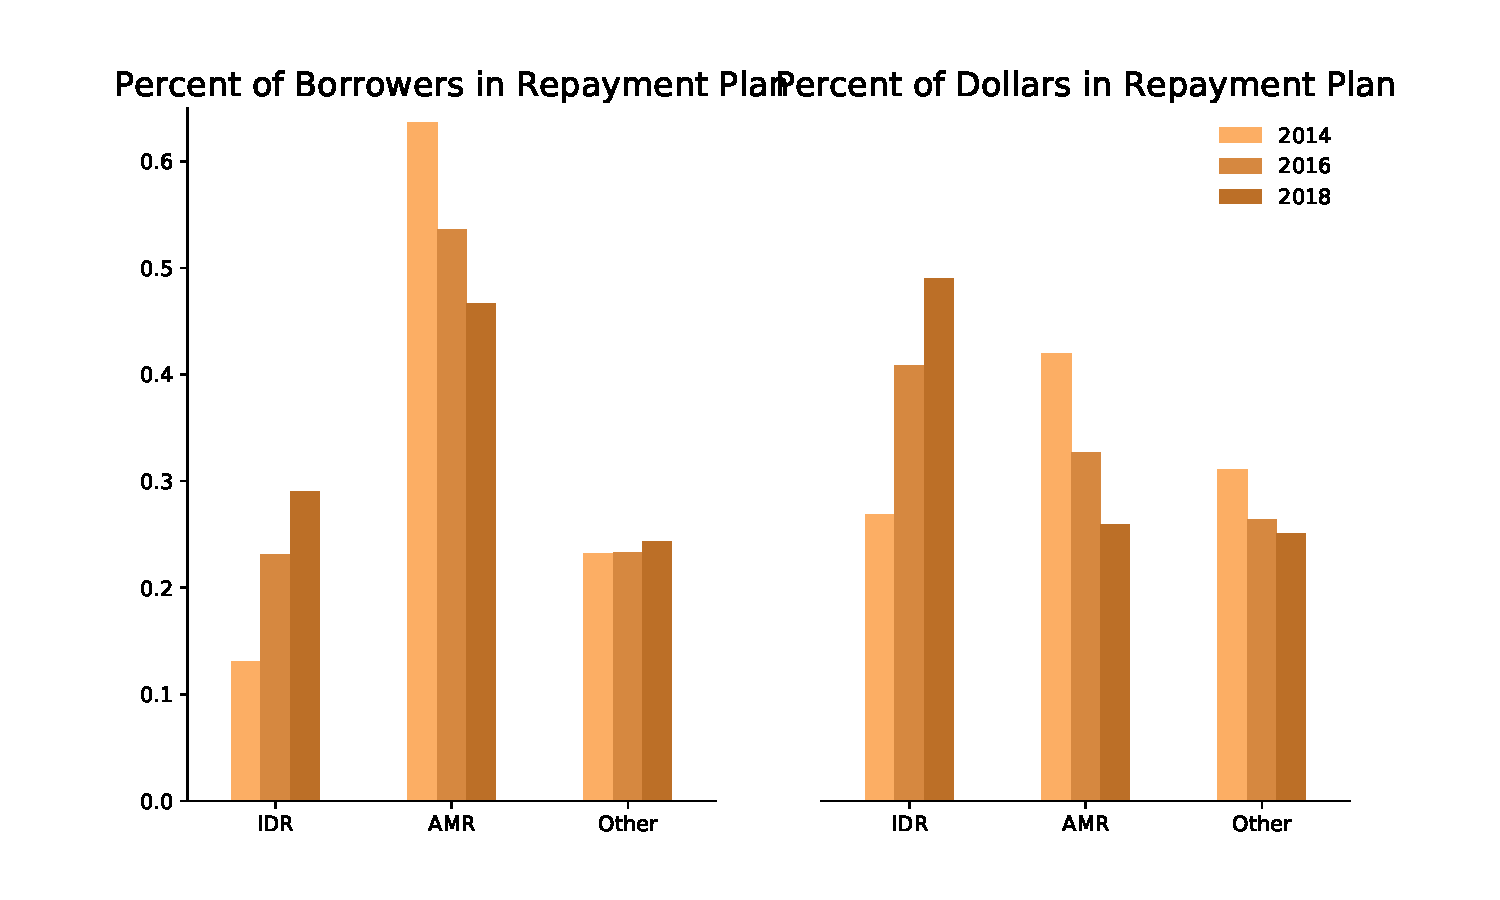
\includegraphics[width=\textwidth]{images/StudentLoans/idr_enrollment_ts.pdf}
      \caption{
        This figure shows how the enrollment in IDR has changed over last 4 years
        \tiny{Source: U.S. Department of Education, Federal Student Aid Data Center, Federal Student Loan Portfolio.}
      }
      \label{fig:idr_enrollment}
    \end{figure}
  \end{center}

  \begin{center}
    \begin{figure}[H]
      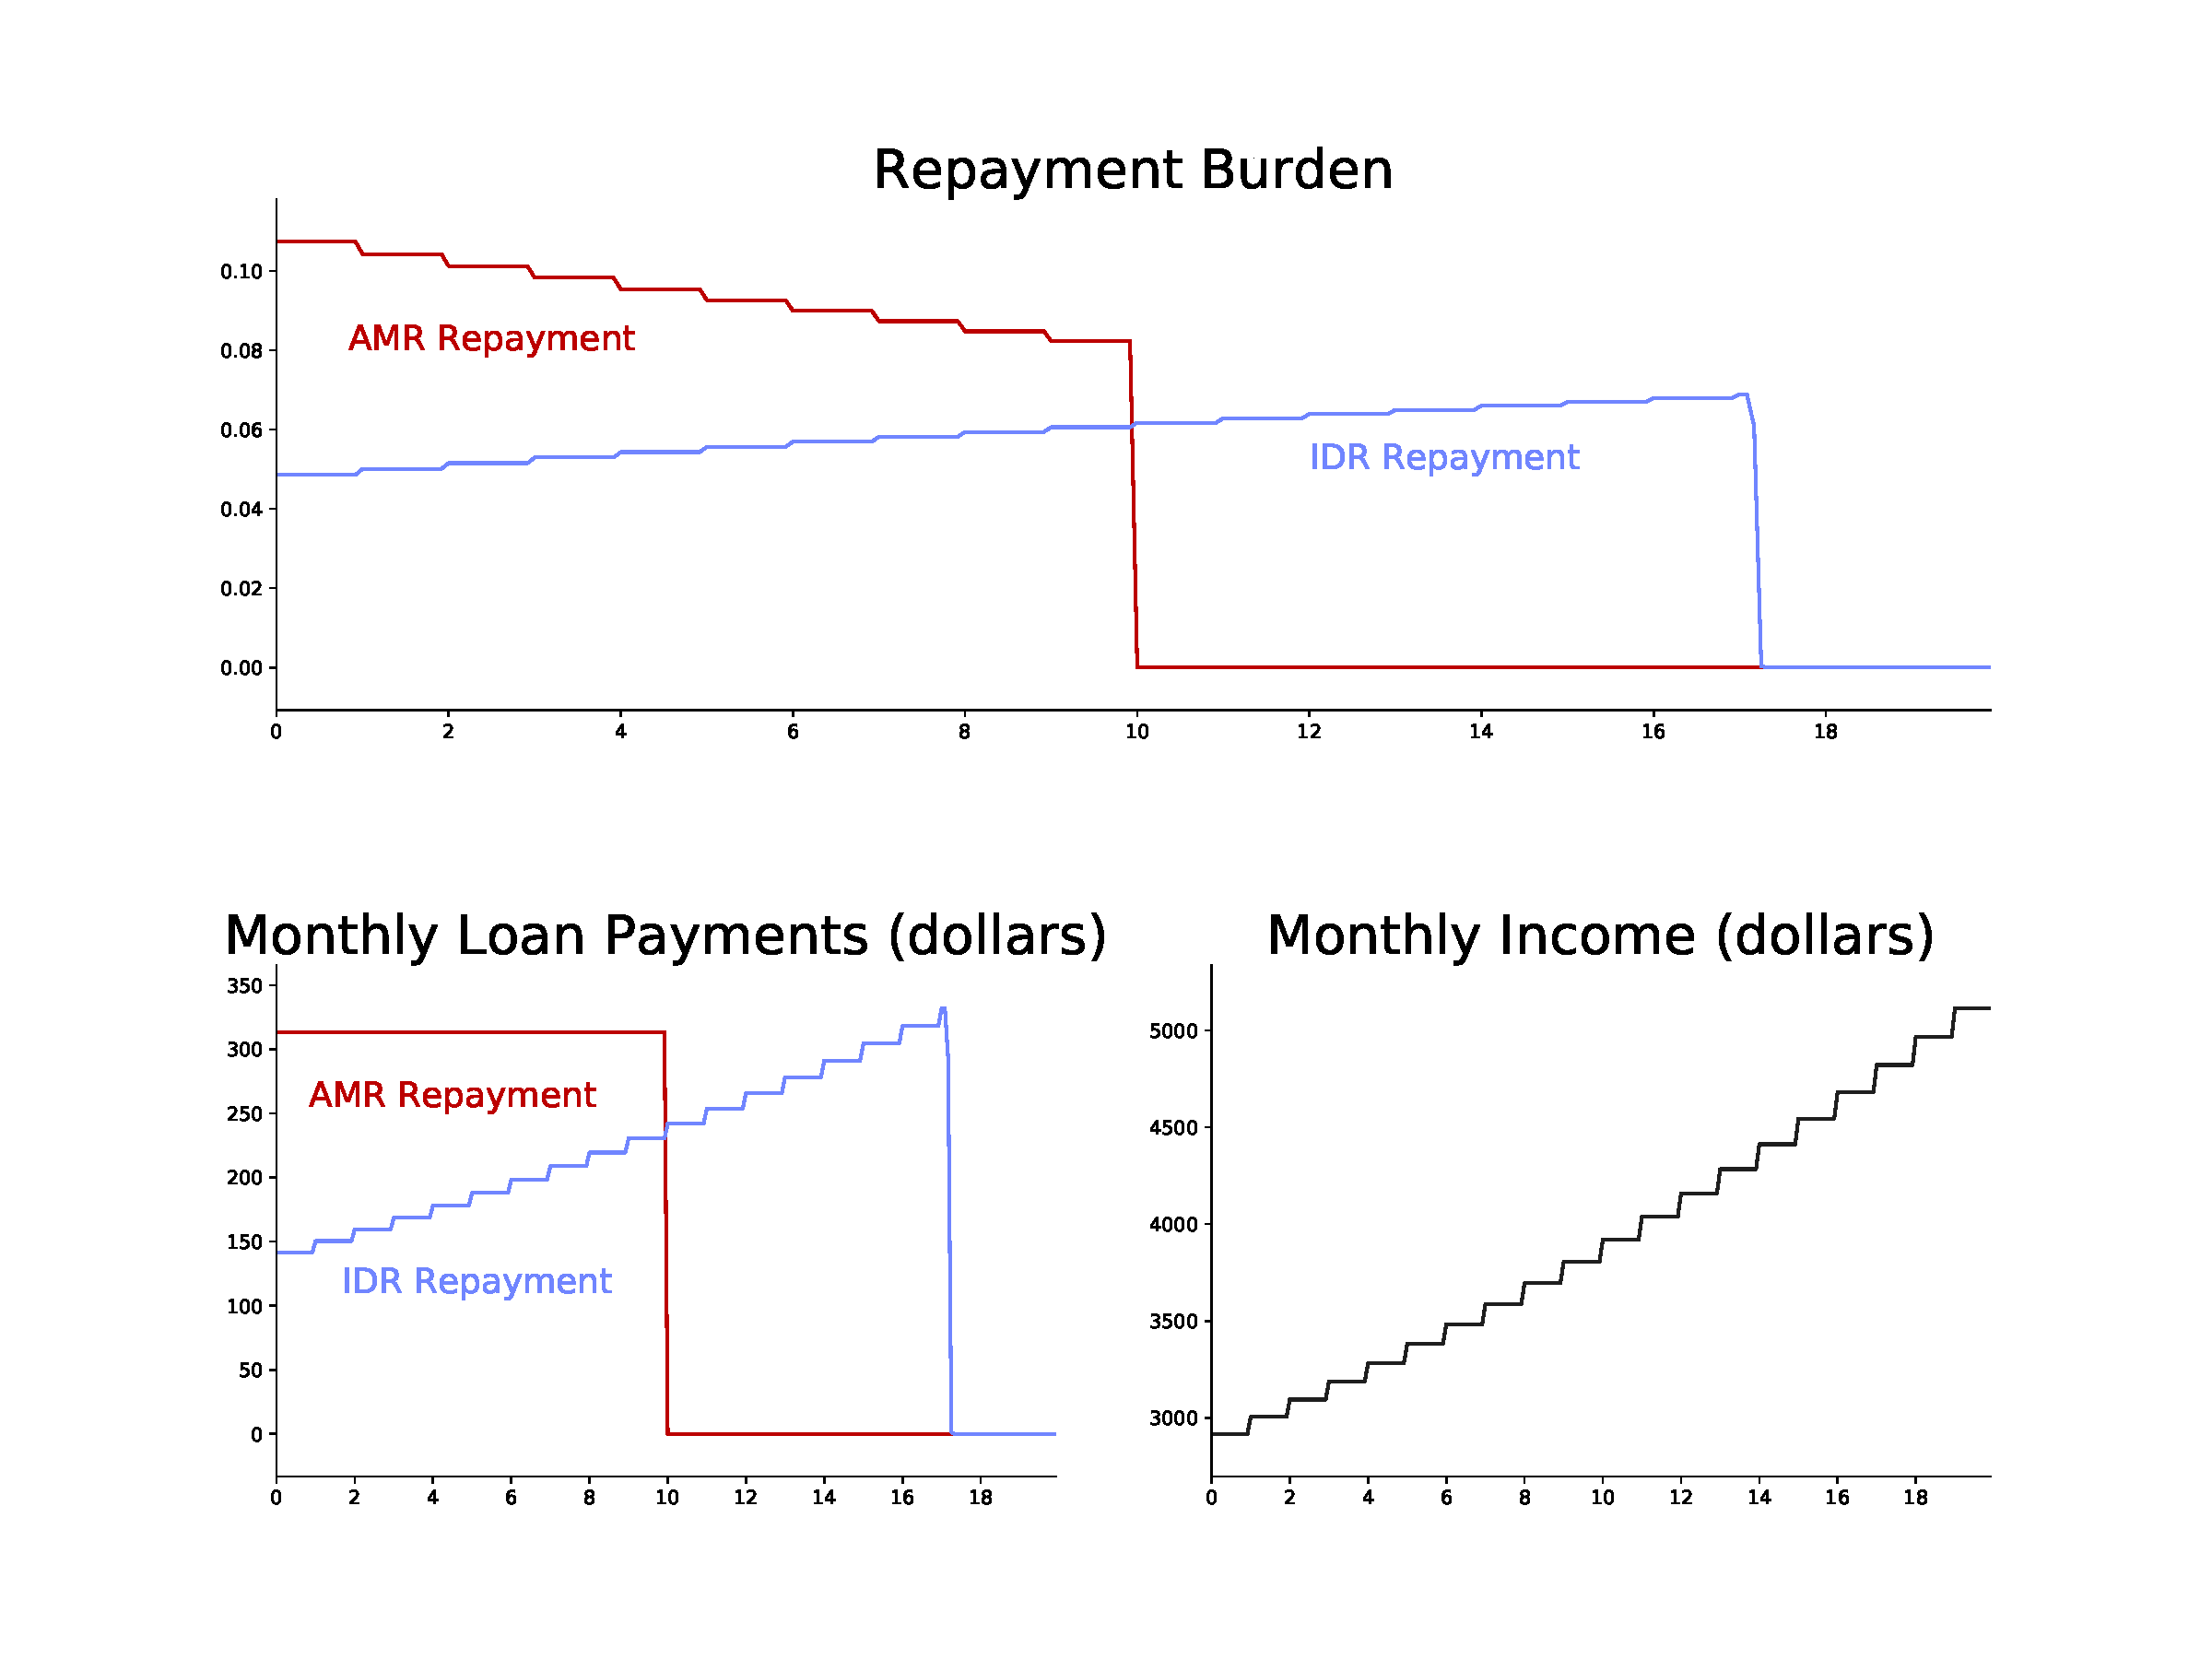
\includegraphics[width=\textwidth]{images/StudentLoans/example_loan_repayment.pdf}
      \caption{
        This figure shows how the repayment burden and repayment amount differ for the AMR
        and IDR student loan repayment plans. It also plots the history of income for the example
        individual.
      }
      \label{fig:loan_repayment}
    \end{figure}
  \end{center}

  \begin{center}
    \begin{figure}[H]
      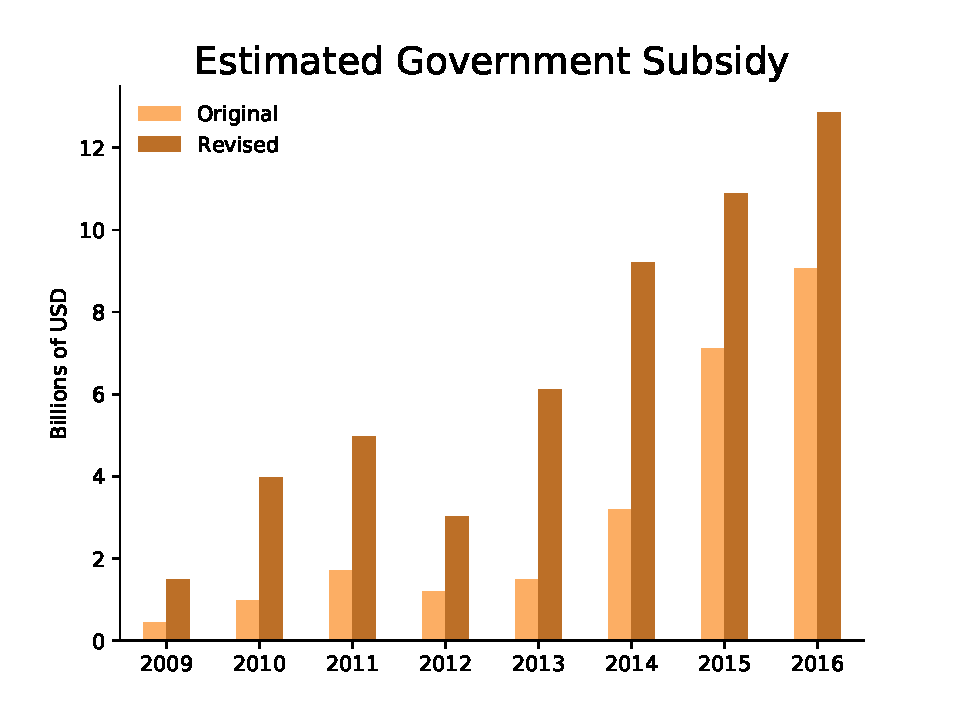
\includegraphics[width=\textwidth]{images/StudentLoans/GovSubsidy_Original_v_Revised.pdf}
      \caption{
        This figure shows the original subsidy estimate alongside the 2017 updated estimate.
        \tiny{Source: GAO analysis of the U.S. Department of Educations' 2011-2017 budget estimates}
      }
      \label{fig:subsidy_original_v_revised}
    \end{figure}
  \end{center}

  \begin{center}
    \begin{figure}[H]
      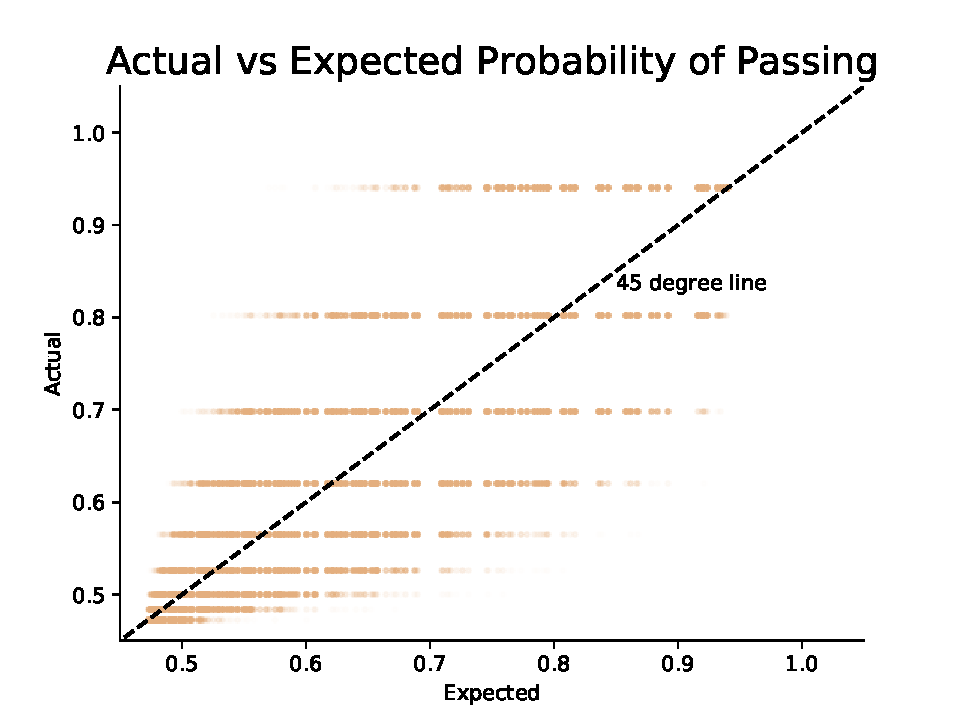
\includegraphics[width=\textwidth]{images/StudentLoans/ep_vs_p.pdf}
      \caption{
        {\small This figure shows the difference between the value function under the IDR and AMR plans for
        a college dropout 3 periods after leaving college. Behind the line is the probability
        distribution over income levels is plotted.}
      }
      \label{fig:scatter_ep_vs_p}
    \end{figure}
  \end{center}

  \begin{center}
    \begin{figure}[H]
      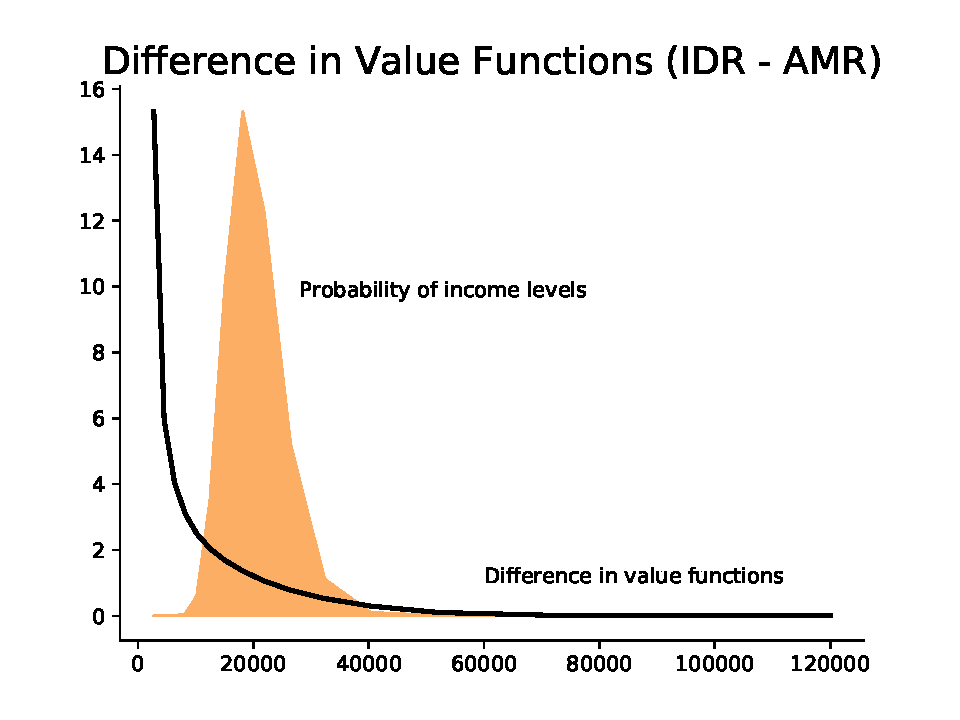
\includegraphics[width=\textwidth]{images/StudentLoans/vf_vs_income_probs.pdf}
      \caption{
        {\small This figure shows the difference between the value function under the IDR and AMR plans for
        a college dropout 3 periods after leaving college. Behind the line is the probability
        distribution over income levels is plotted.}
      }
      \label{fig:vfs_enrollment}
    \end{figure}
  \end{center}

  \begin{center}
    \begin{figure}[H]
      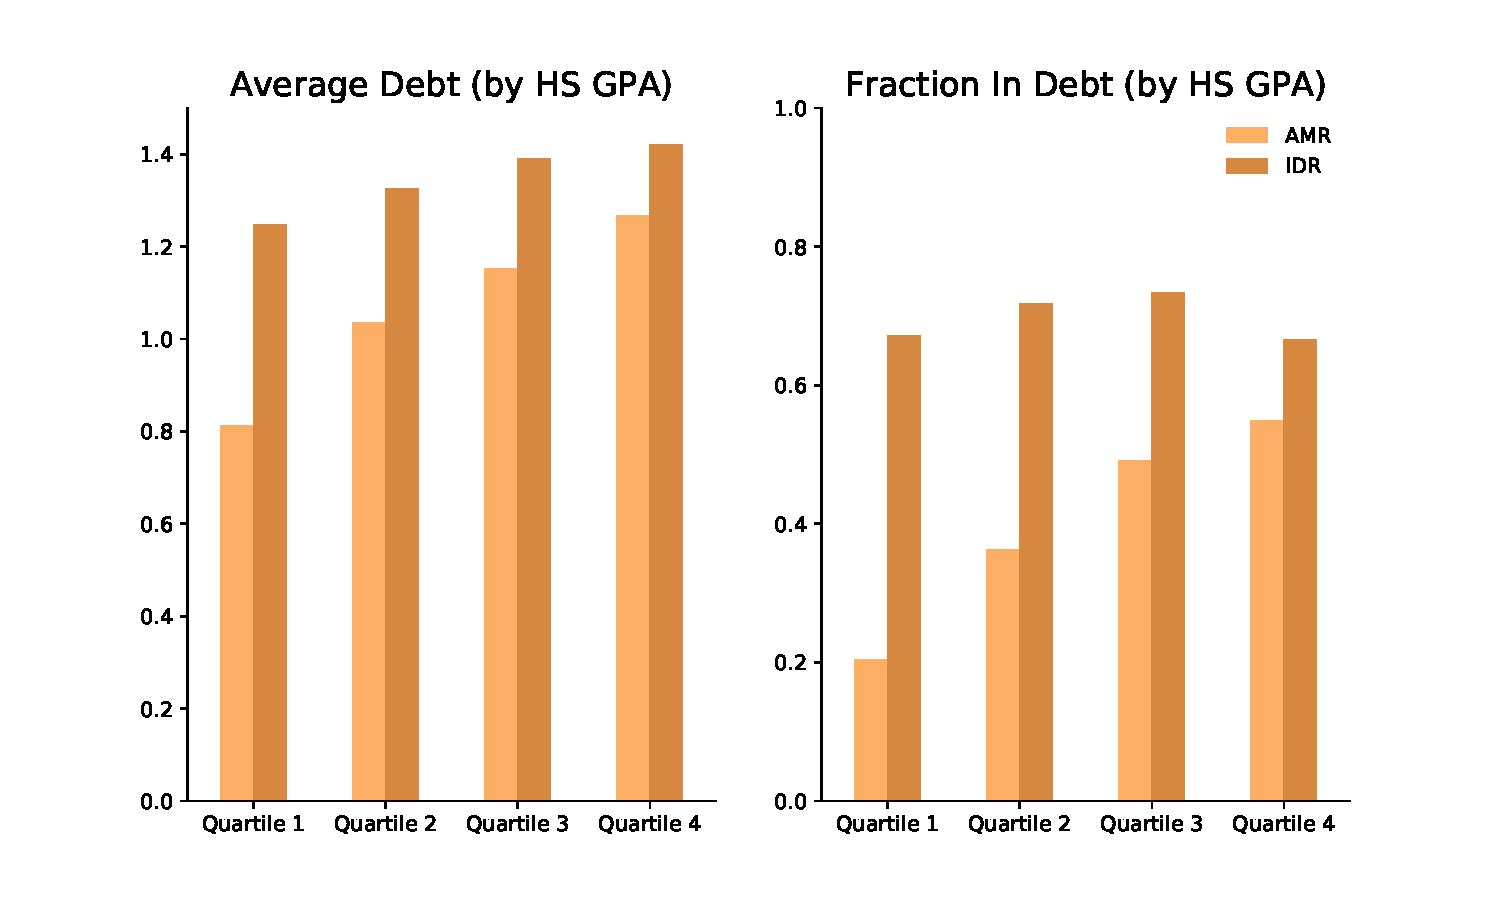
\includegraphics[width=\textwidth]{images/StudentLoans/DebtByGPA.pdf}
      \caption{
        {\small This figure shows the differences in average debt among those who have positive
        student loans and the fraction of college students who borrow for the AMR and IDR plans}
      }
      \label{fig:debt_by_gpa}
    \end{figure}
  \end{center}

  \begin{center}
    \begin{figure}[H]
      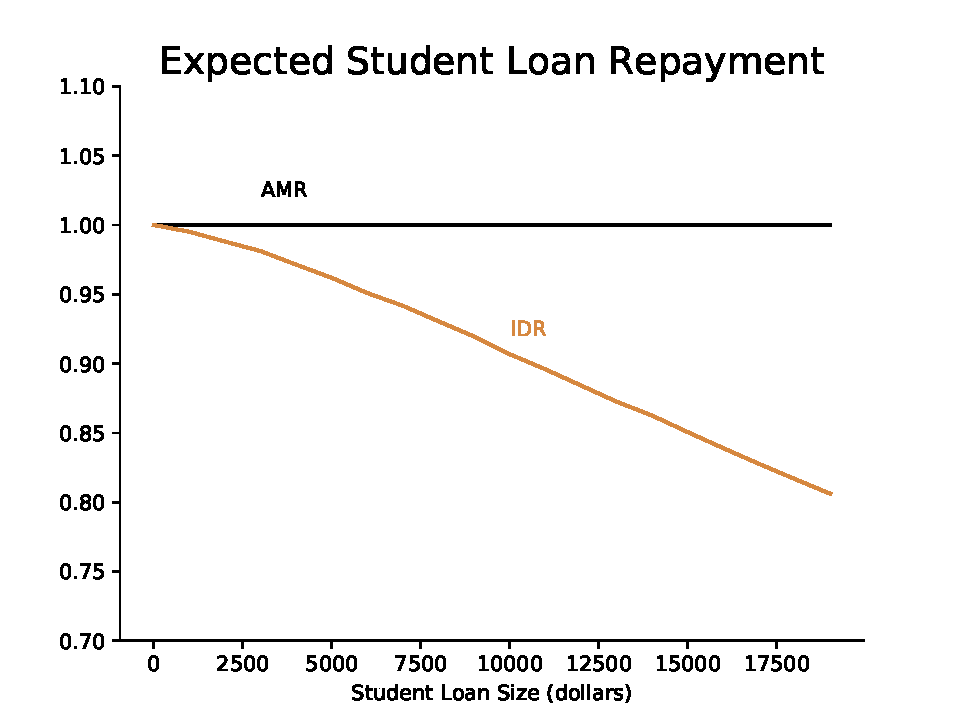
\includegraphics[width=\textwidth]{images/StudentLoans/expected_repayment.pdf}
      \caption{
        {\small This figure shows the fraction of a student loan that is expected to be repaid for
        AMR and IDR across different loan sizes.}
      }
      \label{fig:expected_repayment}
    \end{figure}
  \end{center}
